\label{s:methods}
For a tendon-driven limb with $n$ muscles, the feasible activation space is the unit $n$-cube (As mentioned in the Introduction). As explained in \cite{Valero-Cuevas2009mathematical}, when task constraints are introduced to the system, the feasible activation set is further reduced; in this context, a task is a static force vector produced at the end effector, which is imposed as a constraint on the limb's options in activating its muscles. Thus if this limb meets all constraints, the feasible activation set is given by the polytope $P$ containing all $\textbf{a} \in \mathbb{R}^n$, that satisfy
\[\textbf{f} = A\textbf{a}, \textbf{a} \in [0,1]^n,\]
where $\textbf{f} \in \mathbb{R}^m$ is a fixed output force vector and $A = J^{-T}RF_o \in \mathbb{R}^{m \times n}$--- where $J$, $R$ and $F_0$ are the matrices of the Jacobian of the limb, the moment arms of the tendons, and the strengths of the muscles, respectively \cite{Valero-Cuevas1998Large,Valero-Cuevas2009mathematical}.
The dimensionality of output force $m$ is typically at most 6-dimensional (with force and torque, each in 3 dimensions), and tends to be much smaller than $n$.
$P$ is bounded by the unit $n$-cube since all variables $a_i$, $i \in [n]$ are in the interval $[0,1]$. Each constraint of $\textbf{f}= A \textbf{a}$, is a hyperplane, which has dimension $n-1$.
If $\textbf{f}$ is a feasible submaximal output force, the feasible activation set is a $(n-m)$-dimensional space embedded into the $n$-cube.
Note that in our applications, it is safe to assume that no linear dependencies exist.
Consider the following $1 \times 3$ fabricated example (illustrated in Fig. \ref{fig:schematic_arm}), where the task is a 1 Newton unidimensional force in $x$.
The set of feasible activations is given by the shaded set in Fig. \ref{fig:polygon_slice_solution_space}. Since there are three muscles and one constraint the output space is of dimension $(3-1) = 2$.
Although linearized synergies would be conducive to implement into this model, we do not explore this here.
\begin{align*}
&1 = \frac{10}{3}a_1 - \frac{53}{15}a_2 + 2a_3 \\
&a_1, a_2, a_3 \in [0,1],
\end{align*}

\begin{figure}[h]
  \label{fig:schematic_arm}
  \centering
  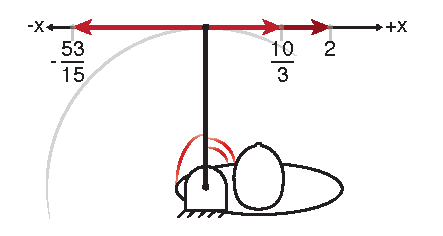
\includegraphics{figs/schematic_arm_1D.pdf}
  \caption{One imagined visualization of the fabricated tendon driven system, with 3 generators.}
\end{figure}

\begin{figure}[t]
  \label{fig:polygon_slice_solution_space}
  \centering
  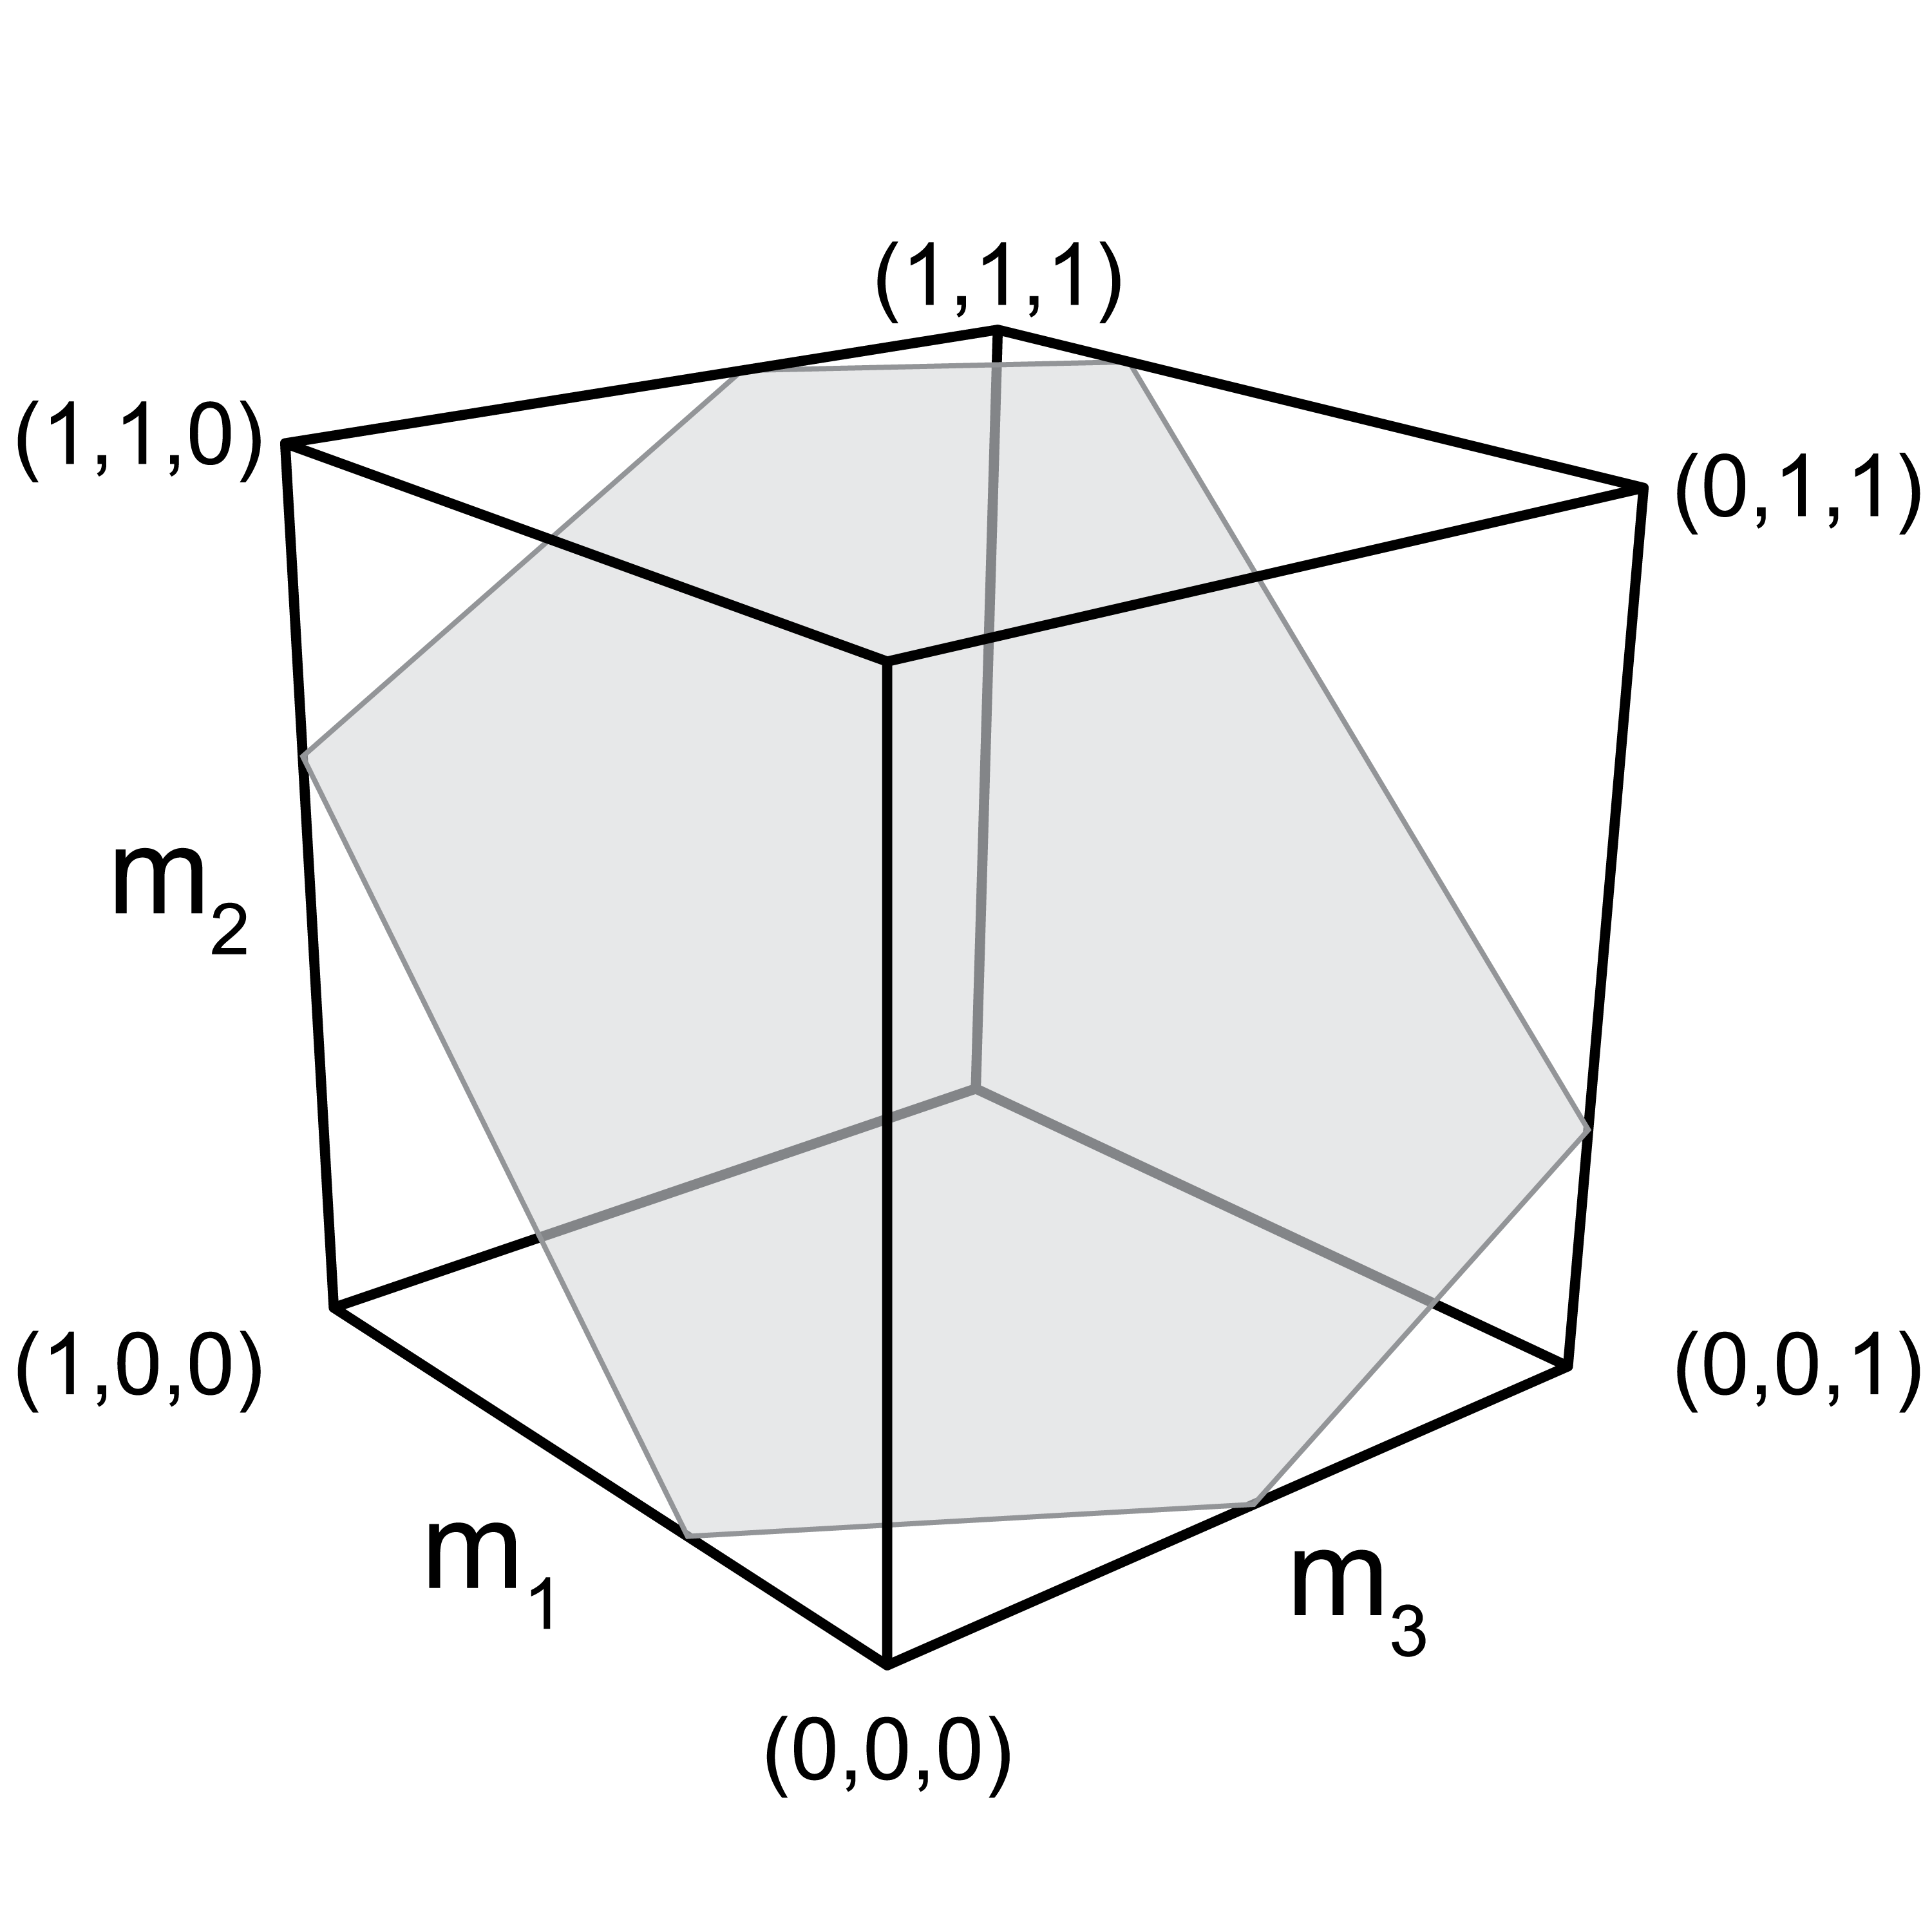
\includegraphics[width=0.25\textwidth]{sections/figs/feasibleactivation.png}
  \caption{The feasible activation set for a  three-muscle system meeting one functional constraint is a polygon in $\mathbb{R}^3$.} %Note that muscle activations are assumed to be bounded between $0$ and $1$.}
\end{figure}

\subsection*{Difficulties of Volume Computation in Higher Dimension}

We are interested in the volume and shape of $P$, but exact volume computations for polytopes is known to be $\#P$-hard \cite{Dyer}.
Several algorithms have been surveyed and implemented, but can only handle small dimensionality, 10 or slightly more \cite{Bueler2}.  
Recent muscle system models we have used have been 31 dimensional \cite{Valero-Cuevas2015high-dimensional}, and other muscle models have over 40 muscles involved \cite{arnold2010model, kutch2012challenges, hamner2010muscle, de2014human}, thereby limiting the feasibility of using direct volume computations. Instead, we chose to uniformly sample the continuous space, effectively approximating the shape of the polytope by calculating point densities.

\subsection*{Hit-and-Run algorithm}
\label{ss:hitrun}
We chose to sample the activation space with the Hit-and-Run method that is known to converge to the uniform distribution across any convex body $K$ \cite{smith1984efficient}.
It is a generalization of a discrete Markov chain, which recursively samples a sequence of points in $K$ as described below.
After $\mathcal{O}^*(n^2R^2/r^2)$ steps, where $r$ and $R$ are the radii of the inscribed and circumscribed ball of $K$ respectively \cite{Dyer, Lovasz}, the Hit-and-Run algorithm has sampled a point uniformly at random (u.a.r.) from the starting point in $K$.
Unfortunately the hidden constant is large, which makes it practically infeasible to obtain the theoretical guarantee of a u.a.r. walk.
Experimental results suggest that a number of points linear with respect to the dimension suffices (as discussed in Section \ref{sec_lengthrun}).
As the feasible activation space of the muscles are given by a convex polytope, this method can be directly applied for our problem.
We chose Hit-and-run because of its easy structure and mixing guarantee; however, it would be interesting to compare Hit-and-Run with the Grid Walk, Ball walk, or other sampling paradigms \cite{Vempala}.

The Hit-and-Run walk on $P$ is defined as follows (it works analogously for any convex body):
\begin{enumerate}
\item Find a starting point $\textbf{p}$ of $P$.
\item Generate a random direction $q$ from $\textbf{p}$ in $P$ (u.a.r. over all directions) (Fig. \ref{fig:hitruncube}a).
\item Find the two intersection points of the line given by the random direction $q$ with the boundary of the polytope (Fig. \ref{fig:hitruncube}b).
\item Choose a point u.a.r.\ on this line segment given by the intersection points (Fig. \ref{fig:hitruncube}c). 
\item Repeat from $2.$ the above steps wit the new point as the starting point, for $s$ iterations until the model is mixed.
\end{enumerate}

\begin{figure}[h]
\centering
\includegraphics[width=0.5\textwidth,page=10]{sections/figs/HitandRunSchematics_all.pdf}
\caption{Graphical description of the Hit-and-Run algorithm.}
\label{fig:hitruncube}
\end{figure}

\begin{figure}[h]
\centering
\includegraphics[width=0.3\textwidth,page=9]{sections/figs/HitandRunSchematics_all.pdf}
\caption{Uniform distribution aross the feasible activation space.\ In the schematic arm example, the distribution is represented within a 2D plane.}
\label{fig:posthitrun_distribution}
\end{figure}

\subsection*{Implementation of Hit-and-Run}
To find a starting point in $P$, the polytope given by
\[\textbf{f} = A\textbf{a}, \textbf{a} \in [0,1]^n,\]
we only need to find one feasible activation vector in the space.
For the Hit-and-Run algorithm to mix faster we don't want the starting point to be close to a vertex of the $n$-cube \cite{Lovasz}.
We use the following standard trick with slack variables $\epsilon_i$, which for applications often gives a good starting point.

\begin{equation}\label{eq:LP_r}
\begin{array}{lrcl}
\mbox{maximize} & \sum_{i=1}^n \epsilon_i \\ 
\mbox{subject to} & \textbf{f} &=& A\textbf{a}\\
  & a_i &\in& [\epsilon_i, 1- \epsilon_i], \hspace{5mm} \forall i \in \{1,\dots,n\}  \\
  & \epsilon_i &\geq& 0, \hspace{5mm} \forall i \in \{1,\dots,n\}.  
\end{array}
\end{equation}


The rest of the implementation of the Hit-and-Run algorithm is straight forward except for the choice of the random direction. How do we sample u.a.r.\ from all directions in $P$? Suppose that $\textbf{q}$ is a direction in $P$ and $\textbf{p} \in P$. Then by definition of $P$, $\textbf{q}$ must satisfy $\textbf{f} = A(\textbf{p}+\textbf{q})$. Since $\textbf{p} \in P$, we know that $\textbf{f} = A\textbf{p}$ and therefore 
\[\textbf{f} = A(\textbf{p} + \textbf{q}) = \textbf{f} + A\textbf{q} \Rightarrow A\textbf{q} = 0. \]

Hence we need to choose directions uniformly at random across the vector space 
\[V = \{\textbf{q} \in \mathbb{R}^n | A\textbf{q} = 0\}.\]

As shown by Marsaglia this can be done as follows \cite{Marsaglia}.
\begin{enumerate}
\item
Find an orthonormal basis $b_1, \dots, b_r \in \mathbb{R}^{n}$ of \{$\textbf{q} \in \mathbb{R}^n | A\textbf{q} = 0$\}.
\item
Choose $(\lambda_1, \dots, \lambda_r) \in \mathcal{N}(0,1)^r$ (from the Gaussian distribution).
\item
$\sum_{i=1}^r \lambda_i b_i$ is a u.a.r.\ direction.
\end{enumerate}
A basis of a vectorspace $V$ is a minimal set of vectors that generate $V$, and it is orthonormal if the vectors are pairwise orthogonal (perpendicular) and have unit length. Using basic linear algebra one can find a basis for $\{q \in \mathbb{R}^n | A\textbf{q} = 0\}$ and orthogonalize with the well known Gram-Schmidt method (for details see e.g.\ \cite{Robertson}). Note that in order to get the desired u.a.r.\ sample the basis needs to be orthonormal. The limb model is defined such that the rows of $A$ are linearly independent and hence $r=n-m$.

\subsection*{Mixing Time}
\label{sec_lengthrun}
From a given starting point, how many iterations of the Hit-and-Run method are necessary to reach a u.a.r.\ point?
For convex polytopes in $n$ dimensions up to $40$, experimental results suggest that $\mathcal{O}(n)$ steps of the Hit-and-Run algorithm are sufficient.
In particular, the paper \cite{emiris2013efficient} by Emiris and Fisikopoulos suggests that $10(n + 1)$ steps are enough to converge upon the uniform distribution \cite{emiris2013efficient}, while in Ge et al.'s paper every single point of the Hit-and-Run algorithm is used in the sample \cite{Ge}. 

\subsection*{Realistic index finger model}
\label{ss:finger}
We used our published model in \cite{Valero-Cuevas1998Large} to find matrix $A \in \mathbb{R}^{4 \times 7}$, where $\textbf{a} \in \mathbb{R}^7$; the four degrees of freedom were ad-abduction, flexion-extension at the metacarpophalangeal joint, and flexion-extension at the proximal and distal interphalangeal joints.
The force direction we simulated are visible in Fig. \ref{fig:finger}.
In this model, for each input we ran 1,000,000 Hit-and-Run iterations and sampled every 100th point- thus generating 10,000 points which are sampled uniformly at random.
To validate the Hit-and-Run algorithm, we computed the theoretical maximum and minimum activation for each muscle for the given force (Fig. \ref{fig:raw_histograms} and \ref{fig:Z_progression}); we found that the difference between the theoretical and observed bounds for all muscles was smaller than 0.001.

\begin{figure}[ht]
  \centering
  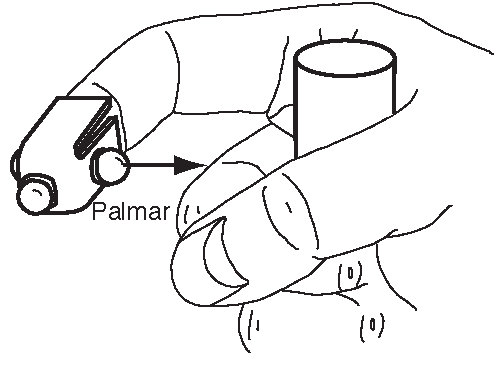
\includegraphics[]{sections/figs/finger.pdf}
  \caption{The index finger model simulated force production in the distal direction. Adapted from \cite{Valero-Cuevas1998Large}.}
  \label{fig:finger}
\end{figure}

\subsection*{Parallel coordinates visualization}
A common way to visualize higher dimensional coordinate data is using parallel coordinates, and has been used in biomechanical studies \cite{bachynskyi2013biomechanical, krekel2010visual}.
To show our sample set of points in the feasible activation space we draw $n$ parallel lines for each of the $n$ muscles.
With the axis labels of the line set between 0 and 1, each point is then represented by connecting their coordinates by $n-1$ lines.
Using an interactive surface we restrict each muscle function to any desired interval- see Fig. \ref{fig:parcoord_full} and \ref{fig:parcoords}.
We decided to simulate a 40\% reduction in activation (feasible tendon force production) in the three index finger muscles innervated by the deep branch of the ulnar nerve- PI, DI, and FDP. 

\subsection*{Muscle-metabolic and neural drive cost functions}

For every solution collected, we used popularly-used cost functions: we computed activation $l_1$, $l_2$ and $l_3$ norms, and the tendon-force $l_1^w$, $l_2^w$ and $l_3^w$ weighted norms.


\begin{table}[h]
\centering
\begin{tabular}{@{}ll@{}}
\toprule
\textbf{Name} & \textbf{Cost function}  \\ \midrule
$l_1$            & $\sum_{i=1}^n a_i$                                     \\
$l_2$            & $\sqrt{\sum_{i=1}^n a_i^2}$                                    \\
$l_3$            & $\sqrt[3]{\sum_{i=1}^n a_i^3}$                                   \\
$l_1^w$            & $\sum_{i=1}^n a_i F_{0i}$                                    \\
$l_2^w$            & $\sqrt{\sum_{i=1}^n (a_i F_{0i})^2}$                                  \\
$l_3^w$            & $\sqrt[3]{\sum_{i=1}^n (a_i F_{0i})^3}$                                    \\ \bottomrule
\end{tabular}
\caption{Cost functions and their usage, where $a_i$ and $F_{0i}$ represent a muscle's activation in a given solution and the maximal musculotendon force, respectively.}
\label{cost_function_tabls}
\end{table}

We added six additional vertical lines, one for each cost function (Table \ref{cost_function_tabls}), to the parallel coordinates plot to show the associated costs of each point. With the same parallel coordinates framework as developed with muscle activation, we can restrict and subset solutions which fall into desired cost-function ranges, thereby masking sub-optimal solutions and highlighting only those meeting the criteria.

\subsection*{Solution projection histograms}
While parallel coordinates are effective in showing the relatedness of muscles in a given task, it is difficult to visually extract the density of the distribution across each individual muscle. Fig. \ref{fig:raw_histograms} shows the activation distribution of each muscle, when activated with $50\%$ of the maximal activation force. The diagram shows, for each muscle, the relative number of solutions that activate the muscle to some range in $[0,1]$ (counted within each histogram break).
We also show the observed activation upper and lower bounds for each muscle (vertical dotted lines).
In Section \ref{sub:activation_spaces_for_increasing_force} we consider the distributions for different forces into distal direction.
\begin{figure}[h]
\centering
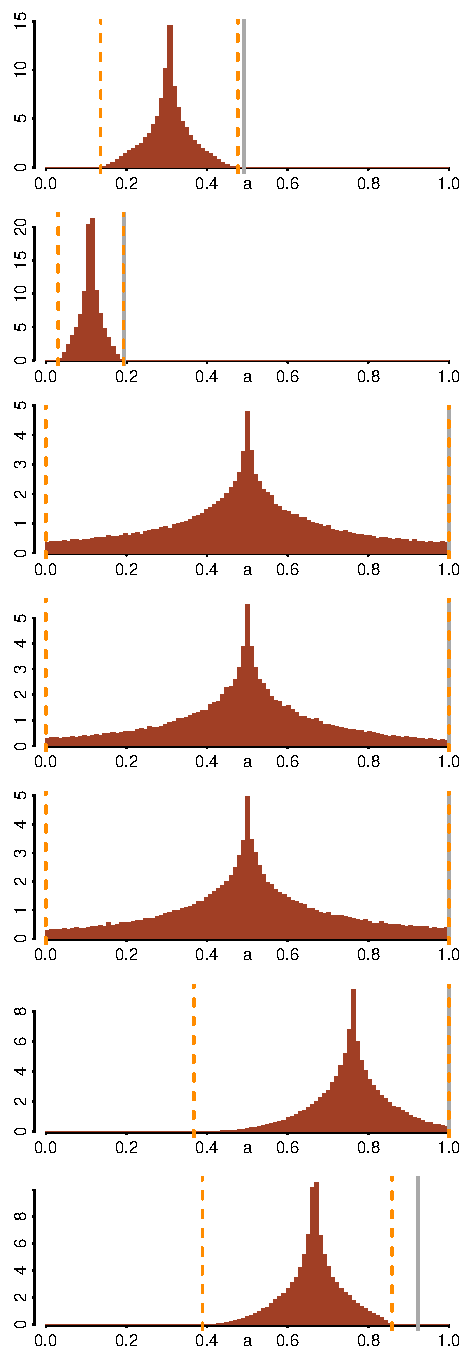
\includegraphics[width=0.5\textwidth]{figs/raw_histograms.pdf}
\caption{Distribution of feasible activations for $\alpha= 0.5$ (50\% of the computed maximal force output in the distal direction). Dashed lines are the observed lower and upper bounds.}
\label{fig:raw_histograms}
\end{figure}


